\documentclass{article}

\usepackage{amsmath,amsthm,amssymb,tikz,float}

\usetikzlibrary{arrows,automata, positioning}

\newtheorem{thm}{Theorem}
\newtheorem{lem}[thm]{Lemma}
\newtheorem{cor}[thm]{Corollary}
\newtheorem{alg}[thm]{Algorithm}

\theoremstyle{definition}
\newtheorem{defn}[thm]{Definition}

\numberwithin{thm}{subsection}

\title{Temporal Graphs Research at Pomona College\\
  \textit{Working Definitions and Vocabulary}
}
\author{Campbell, Wollman, Wu}

\begin{document}

\maketitle

\section{About}

As we continue researching temporal graphs and their related properties there is
an increased need to establish fundamental definitions. Although many papers
have established definitions of the terms and concepts contained within this
paper, there are subtle details of each of these definitions that vary from
paper to paper making it difficult to efficiently communicate exact ideas.

This document shall serve as an ongoing record of the definitions we will use
in our research. The definitions contained within should serve as the defaults
in conversations; if you intend to use an alternate definition to a concept
defined in this document, you should state and/or cite the alternate definition.
(In the future, we will look to incorporate alternate definitions in this
document as well.) It should be noted that these definitions may change as we
continue our research.

\section{Preliminary Definitions}

\begin{defn}
  A \textbf{temporal graph} or \textbf{temporal network}\footnote{We will treat
  the terms \textit{graph} and \textit{network} synonymously throughout this
  paper.} is defined as a tuple $G \in V \times E$ where $V$ is the set of
  vertices, and $E \in V^2 \times T^2$ is the set of edges such that
  $T = [0, \infty)$:

  \[ G = (V, E) \]

  Each edge $e \in E$ is a 5-tuple $(v_i, v_j, t_0, t_f, w)$ such that
  $v_i, v_j \in V$, $t_0, t_f \in T$, and $t_0 \leq t_f$. An edge is said to
  connect $v_i$ to $v_j$ (with the possibility of $v_i = v_j$) between the time
  $[t_0, t_f]$ with weight $w \in W$ with $W \subseteq \mathbb{R}$. That is, all
  edges are to be treated as directed edges with some weight and time-window
  (possibly instantaneous) in which they are \textit{active}. Additionally, we
  will maintain the standard definitions of \textit{size} and \textit{order}
  defined respectively: $|E| = m$,  $|V| = n$.
\end{defn}

With this generalized definition of a temporal network, we will begin to explain
some common, specialized descriptors of these networks:

\begin{defn}
  We will define an \textbf{undirected temporal graph} as a temporal network
  $(V,E^2)$ with $V$ a set of vertices and $E^2$ is a set such
  that $e \in E^2$ is defined to be an unordered pair of 5-tuples

    \[e = \left((u,v,t_0, t_f, w), (v,u,t_0,t_f, w)\right)\]

  with $u,v \in V, t_0, t_f \in [0, \infty],$ and $w \in W$ with
  $W \subseteq \mathbb{R}$. For simplicity, we can describe an edge $e$ as above
  by its first or second 5-tuple, since the existence of one implies the
  existence of the other.
\end{defn}

Note that there is a direct transformation between undirected temporal graphs and
directed temporal networks. To go from undirected to directed, for every edge
$(e_l,e_r) \in E^2$, add edges $e_l \in E$ and $e_r \in E$ to the directed
network. To go from directed to undirected, if for every $u,v$ pair in the
directed network, the number of edges of the form $(u,v,t_0,t_f,w)$ is the same
as the number of edges of the form $(u,v,t_0,t_f,w)$, then pair up these edges;
otherwise there is no transformation.

\begin{defn}
  We will describe a temporal graph as \textbf{unweighted} if every edge in $E$
  has equal weight $w$.
\end{defn}

\begin{defn}
  \textbf{Edge persistence} is the amount of time for which an edge is present.
  More formally, in a graph $(V,E)$ the persistence of an edge $(u,v,t_1,t_2,
  w)$ is defined as $t_2 - t_1$ or simply $\delta t$.
\end{defn}

\begin{defn}
  An edge $e \in E$ is said to be \textbf{infinitely persistent}
  if $t_f = \infty$.
\end{defn}

\begin{defn}
  A \textbf{instantaneous edge} or \textbf{contact edge} is any edge $e \in E$
  where $t_0 = t_f$.
\end{defn}

\begin{defn}
  \textbf{Windowed networks} shall be defined as
  any temporal network where for at least one edge $e = (v_i, v_j, t_0, t_f,w)$,
  $t_0 \neq t_f$.
\end{defn}

\begin{defn}
  \textbf{Contact networks} shall be defined as a temporal network where
  every edge in the network is an \textit{instantaneous edge} or \textit{contact
  edge}. It is simply a special case of an interval network.
\end{defn}

\begin{defn}
  An \textbf{infinitely-edge-persisting network} shall be defined as a temporal
  network where every edge is \textbf{infinitely persistent}.
\end{defn}

\begin{defn}
  A \textbf{co-authorship network} is an undirected interval network in which
  each node represents an author, and the existence of an edge between two nodes
  represents a collaboration over the a period of time $\delta t$. Unless stated
  otherwise, we shall assume a \textit{collaboration} to mean two authors worked
  on $1$ or more publications together in $\delta t$.
\end{defn}

\begin{defn}
  A \textbf{citation network} is a directed interval network $(V,E)$ with
  infinite edge persistence. For simplicity, we can write edges as $u \to_{t_1}
  v$ or $(u,v)_{t_1}$.  In this network, each node represents an author, and the
  existence of an edge $u \to_{t_1} v$ means that author $v$ cited author $u$
  at time $t$. This way the direction of the arrow represents the flow of
  information.
\end{defn}


Now we will move on to consider the different analysis methodologies that will
result from different temporal definitions of `shortest path'.

\begin{defn}
  A graph is a \textbf{path} if it is a simple graph whose vertices can be linearly
  ordered such that there is an edge $uv$ if an only if $u$ and $v$ are adjacent
  in the ordering.
  A digraph is a \textbf{path} if it is a simple directed graph whose vertices
  can be linearly ordered such that there is an edge $u \to v$ if and only if
  $v$ immediately follows $u$ in the ordering.
\end{defn}

\begin{defn}
 A \textbf{shortest path} between $v_1, u$ (di)graph $G = (V,E)$ is
 $P = v_1, v_2, \cdots, v_n, u$ such that $v_i \in V$ for all $i \in [n]$,
 and $v_jv_{j+1}, v_nu \in E$, for all $j \in [n-1]$, and there is no path
 $P' = v_1, v_2, \cdots, v_m, u$ such that $m < n$.
 \end{defn}

Note that this definition does not enforce uniqueness of shortest paths.

\section{Consecutive Contemporaneity}

Here, we consider the addition of paths to include a temporal component, where
any two consecutive edges must share some contemporary period. This is a sensible
definition as two edges should not be able to form a path in a temporal network
if they did not happen at the same time. This is formally defined below.

\begin{defn}
  A \textbf{consecutive temporal path} between $v_1$ and $v_n$ is a path
  $P = v_1, v_2, \cdots, v_n$ such that $v_i \in V$ for all $i \in [n]$,
  and $v_jv_{j+1} \in E$, for all $j \in [n-1]$, and for every pair of
  consectutive edges $(v_{i-1},v_{i})_{t_1}$ and $(v_{i}, v_{i+1})_{t_2}$,
  $t_1 \leq t_2$.
\end{defn}

We will consider the consequences of this definition in the context of different
edge-behaviors, infinite persistence, and windowed persistence.

\subsection{Infinitely Persistent Edges}

The first model we will consider is the simplest of the three, where we disallow
edge-deletion. We will define the persistent coauthorship network to have this
property. [note about semantic equivalence to railway network?]

\begin{defn}
  The \textbf{persistent co-authorship network} a co-authorship network $G = (V,E)$,
  where for all $(u,v,t_1,t_2) \in E$, $t_2 = \infty$. For simplicity, we can
  denote an edge by $(u,v)_{t_1}$ or $u -_{t_1} v$. Since this network is
  undirected, $(u,v)_{t_1} = (v,u)_{t_1}$.
\end{defn}

\begin{figure}[ht] \centering
  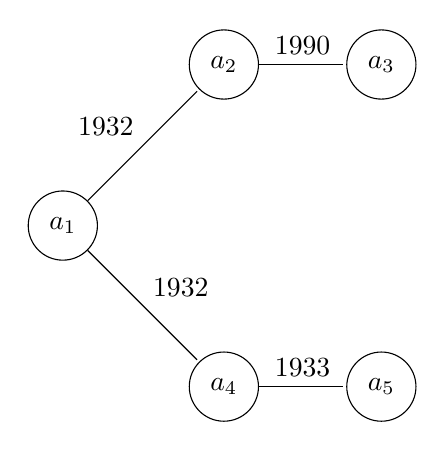
\begin{tikzpicture}[>=stealth',shorten >=1pt,auto,node distance=2cm]
    \node[state]     (a1)                            {$a_1$};
    \node[state]     (a2)     [above right=of a1]    {$a_2$};
    \node[state]     (a3)     [right of=a2]          {$a_3$};
    \node[state]     (a4)     [below right=of a1]    {$a_4$};
    \node[state]     (a5)     [right of=a4]          {$a_5$};

    \path[-]
      (a1) edge             node {1932} (a2)
           edge             node {1932} (a4)
      (a2) edge             node {1990} (a3)
      (a4) edge             node {1933} (a5);
  \end{tikzpicture}
  \caption{Example motivating the difference in shortest vs. fastest path}
  \label{fig:infinite_edge_ex}
\end{figure}

Then, we can consider what a reasonable definition of `shortest path' might be.
In this model, once an edge exists, it is always traversible, so if author
$a_1$ wrote a paper with author $a_2$ in 1932, and author $a_2$ wrote a paper with
$a_3$ in 1990, we can find a path between $a_1$ and $a_3$.  It is also feasible
that $a_1$ wrote a paper with $a_4$ in 1932 as well, and then $a_4$ and $a_3$
wrote a paper in 1933. These two paths $P_1 = a_1 -_{1932} a_2 -_{1990} a_3$, and
$P_2 = a_1 -_{1932} a_4 -_{1933} a_5$ should have some manner of differentation,
since the difference in start times of the edges is 58 in $P_1$ and only 1
in $P_1$. This can be seen in Figure \ref{fig:infinite_edge_ex}, to motivates a
difference in `fastest' vs. `shortest' path.


\begin{defn}

  \label{defn:short_fast_path}

  The \textbf{temporal shortest path} beteween $u$ and $v$ is a consecutive
  temporal path $u,v_1,\cdots,v_n,v$ such there exists no other $u,u_1, \cdots
  u_m,v$ such that $m < n$.

  The \textbf{temporal fastest path} bewteen $v_1$ and $v_n$ is consecutive
  temporal path $v_1,v_2,\cdots,v_n$, with first edge $(v_1,v_2)_{t_1}$ and last
  edge $(v_{n-1},v_n)_{t_{n-1}}$, such that there exists no other
  $u_1,u_2, \cdots, u_m$ with first edge $(u_1,u_2)_{s_1}$, last edge
  $(u_{m-1},u_m)_{s_{m-1}}$ and $s_{m-1} - s_1 < t_{n-1} - t_{1}$.
\end{defn}


\begin{cor}
  Shortest path in persistent coauthorship network is the same as the shortest
  path in the aggregated static graph.
\end{cor}

\begin{proof}[Proof. (Idea)]
  Since the edges have infinite persistence, can just wait at a vertex until
  the desired edge in the aggregated graph shows up.
\end{proof}


\subsection{Windowed edges}

Now consider that we in fact limit the persistence of the edges with an endpoint
specific to each edge (as is specified in the definition of an interval network
temporal graph). We call this graph a \textbf{windowed co-authorship network} or
simply a \textbf{co-authorship network}. If we specify a universal
edge-persistence $\Delta t$ such that for all edges $(u,v,t_1,t_2)$ in the
network, $\Delta t = t_2 - t_1$, then we call this co-authorship network
\textbf{$\Delta t$-windowed}.

When we consider the above definition of a path it is clearly too
simplistic, as it does not consider that an edge may cease to exist. So let
us consider a new definition of a temporal path.

\begin{defn}
  A \textbf{windowed temporal path} bewteen $v_1$ and $v_n$ is a collection of
  edges $(v_1,v_2,s_1,t_1),(v_2,v_3,s_2,t_2), \cdots (v_{n-1},v_{n}, s_{n-1},
  t_{n-1})$ such that $v_1$ and $v_n$ have degree $n$, and the remaining
  vertices have degree 2.  Most importantly, $t_i \geq s_{i+1}$ for all $i \in
  [n-2]$.
\end{defn}

The definitions for fastest and shortest path will be the same as in definition
\ref{defn:short_fast_path}.

\section{Pairwise Contemporaneity}

Here we can consider many of the same definitions, but under are different
lens of contemporaneity for paths. Here we want all edges to have some overlap
in their time interval.

\begin{defn}
  A \textbf{pairwise contemporary temporal path} between $v_1$ and $v_n$ is a
  collection of edges $(v_1,v_2,s_1,t_1), (v_2,v_3,s_2,t_2), \cdots (v_{n-1},
  v_n,s_{n-1}, t_{n-1})$, such that $\bigcap_{i \in [n-1]} [s_i, t_i]
  \neq \emptyset$.
\end{defn}

As might be expected, pairwise contemporary temporal paths behave the same way
that consecutive temporal paths do in the persistent co-authorship network.
Since the edges have infinite persistence, all edges are contemporary `at
infinity.'

In the case of the windowed co-authorship network, the definitions remain the
same for shortest and fastest paths.

\begin{figure}[h] \centering
  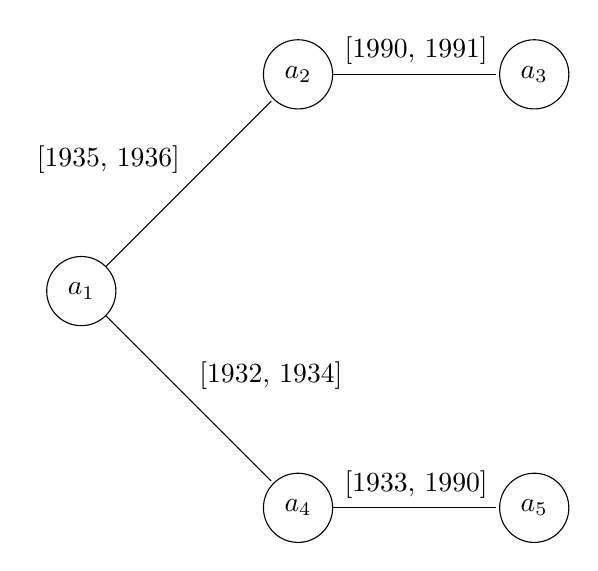
\begin{tikzpicture}[>=stealth',shorten >=1pt,auto,node distance=3cm]
    \node[state]     (a1)                            {$a_1$};
    \node[state]     (a2)     [above right=of a1]    {$a_2$};
    \node[state]     (a3)     [right of=a2]          {$a_3$};
    \node[state]     (a4)     [below right=of a1]    {$a_4$};
    \node[state]     (a5)     [right of=a4]          {$a_5$};

    \path[-]
      (a1) edge             node {[1935, 1936]} (a2)
           edge             node {[1932, 1934]} (a4)
      (a2) edge             node {[1990, 1991]} (a3)
      (a4) edge             node {[1933, 1990]} (a5);
  \end{tikzpicture}
  \caption{Example showing difference in windowed fastest and shortest paths}
  \label{fig:windowed_path_ex}
\end{figure}

In Figure \ref{fig:windowed_path_ex}, there exists a pairwise contemporary path
$P_1$ such that $P_1 = a_5-a_4-a_1$, but there does NOT exist a pairwise
contemporary path $P_2$ such that $P_2 = a_5-a_4-a_1-a_2$.

\end{document}
